\documentclass[thesis.tex]{subfiles}
\begin{document}

\chapter{SpeedCam}\label{chap:main}

This chapter will describe the three following parts. At first it will outline the general idea of the SpeedCam approach for any network type. After this it will describe the specific adaptation for the SCION network. At last there will be an explanation what has to be changed for SCIONLab and the reason for that.

\section{Overview}
SpeedCam is an heuristic approach to monitor network traffic with regards to limited resources. It analyses the network structure and decided based on the heuristic where are good places to monitor local traffic. The approach also tries to reduce the necessary amount of probes to minimize the resource impact an the machines.


\section{Inspection game}
The idea behind SpeedCam is based on the \textit{Inspection Game} in the game theory \todo{Quelle einfügen}. Inside the game is a \textit{task} to be done under defined \textit{rules}. The execution of the task can be simpler, more efficient or more effective with a violation of these rules. The task is performed by one of the two parties, the \textit{inspectee} and the compliance of the rules costs resources and is monitored by the second party, the \textit{inspector}. The inspectee has a general interest to break the rules to perform better, while the inspector wants to reduce his amount of inspections to use as few as possible resources. The possible combination are shown in \autoref{tab:inspectionGameMatrix}.

\begin{table}[h]
    \centering
    \begin{tabular}{cc|c|c|}
        & \multicolumn{1}{c}{} & \multicolumn{2}{c}{Inspector}\\
        & \multicolumn{1}{c}{} & \multicolumn{1}{c}{Inspect}  & \multicolumn{1}{c}{Ignore} \\\cline{3-4}
        \multirow{2}*{Inspectee}  & Comply & $A$ & $C$ \\\cline{3-4}
        & Violate & $B$ & $D$ \\\cline{3-4}
    \end{tabular}
    \caption{Inspection game matrix.}
    \label{tab:inspectionGameMatrix}
\end{table}

The cases $B$ and $C$ are good investments of the inspectors limited resources. In the first one he didn't inspect while the task was performed without violation and in the second one the inspector found the culprit. For case $A$ were the resources of the inspector wasted because there was no reason to inspect. The inspector failed in its task in case $D$, because he missed a violation of the rules by not investing the resources.

Because of the shown cases and it results it is obvious that a \textit{pure strategy} doesn't make sense in this game. When the inspector always inspect he will waste resources and when the inspector always ignores he fails his task. Instead of a pure strategy there must exist a \textit{mixed strategy} defined by probabilities for each action to be chosen. \todo{Quelel für Nash Beweis}.


\section {Generalized concept} \label{sec:main:generalconcept}
The previously described form of the Inspection game is adopted for networks for this work. The \textit{nodes} of a network are the \textit{inspectees}, their \textit{task} is to \textit{transfer} many data in a short time. The \textit{rule} for all nodes is, that a transaction of data \textit{mustn't exceed the link limits} or disturb other nodes transfer. These limits can be given by the physical cable nature or are artificial bilateral agreed limits. A \textit{detected violation} of these rules can result in throttling the bandwidth or even exclude the node from the node, temporary or permanently. A node can try to exceed the limits and so breaking the rule, while avoiding any inspection. 

The \textit{inspector} in such a game has the possibility to monitor a nodes network traffic. Monitoring a node costs computation resources such as memory or cpu cycles\todo{Quelle für Leistungsaufwand von switches nur für switching}. Both can be critical for a switch to send packets. Therefore an inspection, necessary or not, will have an impact on the network throughput. The challenge of the inspector is to only monitor when a node is exceeding its limits. He will be presented in this work as the SpeedCam approach. These will give the inspector an heuristic with the goal to increase the amount of cases for $B$ and $C$ and to reduce it for $A$ (not wasting resources) and $D$ (fairness for network member).

The general concept of SpeedCam applies to types of networks which meet the following requirements. The network must consist of \textit{nodes}, ASes, and \textit{links}, which connect only two ASes. The nodes and links must form an undirected graph. For SpeedCam it is not necessary that the graph must be known in the first place nor to be static. This is important because real networks tend to be dynamic and to be decentralized with only partial knowledge about its structure. The inspector must have access to these network in such a form, that he can gain knowledge about the networks structure and monitor a nodes traffic.

When the requirements are met the inspector can be run as a component. He executes the SpeedCam approach and stores the necessary information about the nodes. It is described in this work as a centralized component, but it can be split into multiple inspectors each responsible for a subnetwork. 

One run of the SpeedCam approach is called an \textit{episode} and is broken down in four phases, as shown in \autoref{fig:main:phasesOrder}.

\begin{figure}[!h]
	\centering
	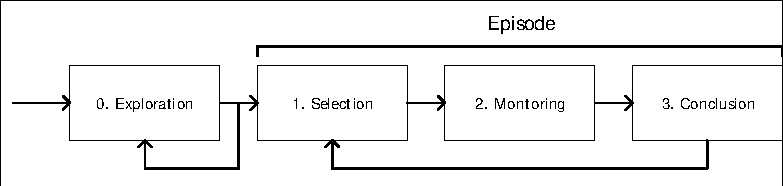
\includegraphics[trim=5mm 1mm 0mm 1mm, clip, width=0.95\textwidth]{umldiagram_phasesOrder.pdf}
	\caption{SpeedCam's phases}
	\label{fig:main:phasesOrder}
\end{figure}


The exploration phase is the 0-th phase because it can be skipped if the network is static and fully explored. This phase can also be running in the background in parallel to the other phases. Phase 1 to 3 must be run in sequential order, because they depend on each other results. The next sections will explain each phase in detail.

\subsection{Exploration} \label{sec:main:explorationphase}
This phase has the goal to create an undirected graph of the network to monitor. The structure of the network is necessary for the following phases. 

For the general concept of the SpeedCam approach exists multiple possibilities to explore the underlying network. Because the only assumption about the network is that nodes are connected via links these possibilities are also general and has some flaws. In later discussed specialized forms of the SpeedCam approach there are fewer flaws.

The first possibility is to manually create the graph. A network, virtual or physically present, must be created by an entity, be it a humanoid administrator or a program. Every change of the network can be logged and used to create the graph. This is obviously a tedious task and not error prone. 

Another possibility needs a start point inside the network. With such a start point it is possible to get all connected nodes with the use of a traversal algorithm, like Breadth-First, Depth-First, Djikstra or Floyd–Warshall. This is for example used by the Border-Gateway-Protocol (BGO).\todo{Quellen für alles}. This is for such a general network the way to explore the network graph.

The exploration phase itself needs to be constantly repeated to react to changes inside the network. Inactive or disconnected nodes doesn't need to be monitored.

\subsection{Selection} \label{sec:main:selectionPhase}

Based on the results of the previous exploration phase, the selection phase uses the network information and returns a set of nodes to monitor. This phase uses the heuristic. It has to estimate in advance if the node will transfer any traffic.

The selection process has two goals to achieve. It has to minimize the amount of used probes to save resources. But also the probes have to form the maximum amount of traffic cover to achieve a high accuracy of the monitoring. These two goals are contradictory. The minimum of probes is zero, which is equals to no inspection and results in no traffic monitored. On the other hand, the complete traffic can be monitored by using all nodes as probes, but this is not resource efficient.

Because of this, the selection heuristic must achieve a trade-off between as few probes as possible with a high enough precision of the monitored traffic. The heuristic will use information about the graph structure itself and information from past monitoring phases to increase the quality of a selection.

The quality of a selection will be defined as the following:

\begin{equation} \label{equo:qualitySelection}
q(S,N) = \frac{\text{traffic}(S)}{\text{traffic}(N)}
\end{equation}
where:
\begin{conditions}
    S     &  Set of probe nodes \\
    N     &  Set of all nodes
\end{conditions}

Another criteria of this phase is the randomness of the selection process. The inspector mustn't be predictable for the inspectees, otherwise they will have an advantage and can avoid an inspection. When a set of probes is predictable for the inspectees, they can decide to violate the rules outset of this set and chose other paths or times to transfer their data. 

For example, the \autoref{fig:intro:exampleMultipath} shows a simple network. Lets assume, that the inspector is watching the node \textbf{1-2} and all the nodes inside the network are knowing this fact. With that knowledge, they will choose the path 1-1$\rightarrow$1-3$\rightarrow$1-4 instead and avoid the inspection. This problem is even more present for a real network, because they tend to be complex and provide even more alternative routes to avoid an inspection.

One solution to counter the predictability is to keep the algorithm and its configuration secret from the inspectees. The solution has two main flaws: The first one is, that \textit{security-by-obscurity} doesn't work in long time. \todo{Quelle für beispiele}. Without going into detail about security problems, there is one weak spot in the security chain, the human itself. A dissatisfied employee can publish the algorithm and its configuration to the public as an act of revenge, sell the information or unintentionally leak it. The other flaw is, that given a big enough sample rate, the insectess can statistically reverse-engineer the algorithm. \todo{Quelle für solche angriffe}

A better solution is to introduce an entropy to the selection process. Instead of using the set with the highest quality, the algorithm will randomly choose a set. This disagrees with the selection process itself. There is no need to select candidates based on information when every candidate can be chosen randomly.

The SpeedCam approach uses a candidate score $cs(n)$ to determine the probability of each node to be chosen. While not guaranteed to be chosen, the chance to be a probe is higher for a good candidate than for a bad candidate. This process will result in a high quality while also being not fully deterministic. The following will describe how this candidate score is composed of.

\subsubsection{Criteria} \label{sec:main:selectionPhase:criteria}
The following presented criteria are considered \textbf{static} and can be calculated without a history of past measurements. They require the topology of the network.

\textbf{Degree} [ $deg(n)$ ]: The sum of incoming and outgoing links of node. This criteria represents the potential for a good transfer hub and can be used by other nodes as a central transfer hub. The higher the degree of a node, the higher the possibility to monitor a great range of traffic sources. A node on the edge of the network, a sink, has a low degree, mostly 1. These are uninteresting because they can only monitor the traffic of this node. A good real example for a node with a high degree are the nodes of submarine cables, as shown here\footnote{\url{https://www.submarinecablemap.com}, 02.04.2018}. They have the ability to connect two continents with each other and provide so a good point to measure traffic.

\textbf{Total capacity} [ $cap(n)$ ]: The sum of the connection capacity of a node. The capacity is the physical or between partners agreed limit to transfer bytes per second. This is similar to the \text{Degree}, but it differs in one aspect: The degree is only a indicator about the possible connectivity, but not for the possible throughput of traffic. A node with a high capacity can be preferred over a node with a high degree and lower capacity to transfer data. Because of this difference the two criteria are separate.

The now following criteria are \textbf{dynamic} and requires a history of the past episodes. The amount of hold episodes is limited by the size of the network, because is needs memory per node. As seen later, the length of saved history will also have an impact on the quality of the selection process.

\textbf{Average activity} [ $\overline{act_{t_1,t_2}}(n)$ ]: The relation between possible and used capacity of a node in a time interval between $t_1$ and $t_2$. The time span can be of any resolution, but should be consistent. 

\begin{equation}
\overline{act_{t_1,t_2}}(n) = \frac{\text{traffic}_{t_1,t_2}(n)}{cap(n)}
\end{equation}

Storing the timespan for an episodes gives the possibility creating a profile for a node to be used by the selection process. The selection itself can now be time based. A node with a high activity in the morning can receive a higher candidate score than a node with a high activity in the evening. This can increase the quality of the set.

The meaningfulness of that criteria depends of the length of the history. A short history maybe represents a inaccurate result of the node, while a long history can hold outdated information about the behaviour of that node. The evaluation part will show the influence of the amount of episodes.

\subsubsection{Candidate score}

The score for each node is calculated as the following:

\begin{equation} \label{equo:candidateScore}
cs(n) = w_{deg}\cdot deg(n) + w_{cap}\cdot cap(n) + w_{act}\cdot \overline{act_{t_1,t_2}}(n)
\end{equation}

where:
\begin{conditions}
    n           &  A node \\
    w_{deg}     &  Weight for the degree,   $\in \mathbb{R}_{\ge 0}$ \\
    w_{cap}     &  Weight for the capacity, $\in \mathbb{R}_{\ge 0}$  \\
    w_{act}     &  Weight for the activity, $\in \mathbb{R}_{\ge 0}$ 
\end{conditions}

The weights are a possibility to configure the algorithm for the needs of a network. The evaluation part will show the results of using different values.

The \textbf{average activity} will be zero for the first episode, because the inspector does not have information about the traffic of such a node.  

\subsubsection{Probability}

The probability to be selected as a SpeedCam depends on the previously calculated candidate score, $cs(n)$ \autoref{equo:candidateScore}. It is calculated for all nodes inside the network and assigned to the node itself for that episode. With that information, the probability can be calculated and assigned to the node with:

\begin{equation}
P_{sc}(n) = \frac{cs(n)}{\text{max}(cs(N))}
\end{equation}
where:
\begin{conditions}
    N           &  All nodes inside the network 
\end{conditions}

\subsubsection{SpeedCam amount}

Now exists a list of candidates with an assigned probability to be selected based on their candidate score. The phase must now select $k$ \textit{SpeedCams} from this set. The size of $k$ should scale with the network size $|N|$, but as discussed earlier it should be as small as possible. There are a few scales, which were inspected in this work:

\textbf{Constant} [ $K$ ]: A constant amount of nodes will be selected, ignoring the size of the network. This is usable for static networks, where $|N|$ is known and does not change, but that applies only to very few networks\todo{quelle dafür finden}. Because of this, a constant value for K will not be evaluated in this work.

\textbf{Logarithmic} [ $log(|N|)$ ]: A logarithmic amount of SpeedCams will scale nicely with any network and it was the first idea for this approach. After the first tests it was shown, that too few SpeedCams were operating and the accuracy of the monitoring was too low. This will be show in \autoref{chap:eva}.

\textbf{Linear} [ $x\cdot |N|, 0 \leq x\ll1$ ]: A linear amount of SpeedCams will need more resources as the logarithmic approach, but will also raise the accuracy to sufficient levels.\todo{Umschreiben!} The factor $x$ must be much-less than 1, otherwise the inspector will utilize half the network and this contradicts the goal to use as few resources as possible. The evaluation will use $x=0.1$, $x=0.2$ and $x=0.33$.

The difference scale effects are visualized in \autoref{fig:main:concept:scaling}. It represents the SCIONLab ISDs 1 and 2 in its current state. A red circle indicates, that this node is selected. The top row from a) to c) shows a network of ten nodes, while the bottom row from d) to f) expands this networks to 16 nodes. 

\begin{figure}
	\centering
	\begin{subfigure}{.3\linewidth}
		\centering
		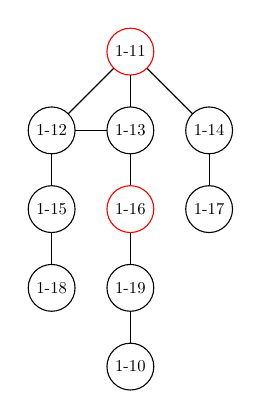
\begin{tikzpicture}
			\tikzstyle{AS}=[circle,draw=black,scale=0.6]
			\begin{scope}
			\node[AS,draw=red] (1-11) at (0,0)   {1-11};
			\node[AS] (1-12) at (-1,-1) {1-12};
			\node[AS] (1-13) at (0,-1)  {1-13};
			\node[AS] (1-14) at (1,-1)  {1-14};
			\node[AS] (1-15) at (-1,-2) {1-15};
			\node[AS,draw=red] (1-16) at (0,-2)  {1-16};
			\node[AS] (1-17) at (1,-2)  {1-17};
			\node[AS] (1-18) at (-1,-3) {1-18};
			\node[AS] (1-19) at (0,-3)  {1-19};
			\node[AS] (1-10) at (0,-4)  {1-10};
			\end{scope}
			
			\path[-]    
			(1-11) edge (1-12) 
			(1-11) edge (1-13)
			(1-11) edge (1-14)
			(1-12) edge (1-13)
			(1-12) edge (1-15)
			(1-13) edge (1-16)
			(1-14) edge (1-17)
			(1-15) edge (1-18)
			(1-16) edge (1-19)
			(1-19) edge (1-10)
			;
		\end{tikzpicture}
		\caption{Constant K=2, k=2}
		\label{fig:main:concept:scaling:const1}
	\end{subfigure}
	\hfill
	\begin{subfigure}{.3\linewidth}
		\centering
		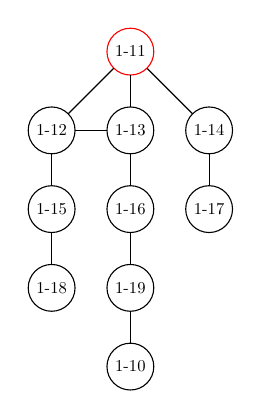
\begin{tikzpicture}
			\tikzstyle{AS}=[circle,draw=black,scale=0.6]
			\begin{scope}
			\node[AS,draw=red] (1-11) at (0,0)   {1-11};
			\node[AS] (1-12) at (-1,-1) {1-12};
			\node[AS] (1-13) at (0,-1)  {1-13};
			\node[AS] (1-14) at (1,-1)  {1-14};
			\node[AS] (1-15) at (-1,-2) {1-15};
			\node[AS] (1-16) at (0,-2)  {1-16};
			\node[AS] (1-17) at (1,-2)  {1-17};
			\node[AS] (1-18) at (-1,-3) {1-18};
			\node[AS] (1-19) at (0,-3)  {1-19};
			\node[AS] (1-10) at (0,-4)  {1-10};
			\end{scope}
			
			\path[-]    
			(1-11) edge (1-12) 
			(1-11) edge (1-13)
			(1-11) edge (1-14)
			(1-12) edge (1-13)
			(1-12) edge (1-15)
			(1-13) edge (1-16)
			(1-14) edge (1-17)
			(1-15) edge (1-18)
			(1-16) edge (1-19)
			(1-19) edge (1-10)
			;
		\end{tikzpicture}
		\caption{Logarithmic, b=10}
		\label{fig:main:concept:scaling:log1}
	\end{subfigure}
	\hfill
	\begin{subfigure}{.3\linewidth}
		\centering
		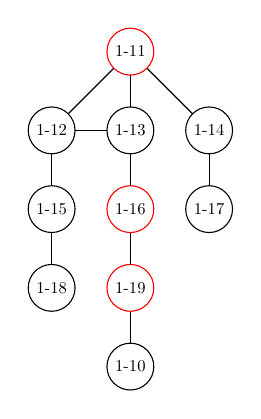
\begin{tikzpicture}
			\tikzstyle{AS}=[circle,draw=black,scale=0.6]
			\begin{scope}
			\node[AS,draw=red] (1-11) at (0,0)   {1-11};
			\node[AS] (1-12) at (-1,-1) {1-12};
			\node[AS] (1-13) at (0,-1)  {1-13};
			\node[AS] (1-14) at (1,-1)  {1-14};
			\node[AS] (1-15) at (-1,-2) {1-15};
			\node[AS,draw=red] (1-16) at (0,-2)  {1-16};
			\node[AS] (1-17) at (1,-2)  {1-17};
			\node[AS] (1-18) at (-1,-3) {1-18};
			\node[AS,draw=red] (1-19) at (0,-3)  {1-19};
			\node[AS] (1-10) at (0,-4)  {1-10};
			\end{scope}
			
			\path[-]    
			(1-11) edge (1-12) 
			(1-11) edge (1-13)
			(1-11) edge (1-14)
			(1-12) edge (1-13)
			(1-12) edge (1-15)
			(1-13) edge (1-16)
			(1-14) edge (1-17)
			(1-15) edge (1-18)
			(1-16) edge (1-19)
			(1-19) edge (1-10)
			;
		\end{tikzpicture}
		\caption{Linear, x=0.33}
		\label{fig:main:concept:scaling:lin1}
	\end{subfigure}
	
	\begin{subfigure}{.3\linewidth}
		\centering
		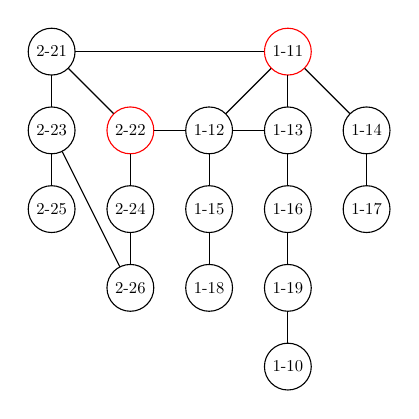
\begin{tikzpicture}
			\tikzstyle{AS}=[circle,draw=black,scale=0.6]
			\begin{scope}
			\node[AS,draw=red] (1-11) at (0,0)   {1-11};
			\node[AS] (1-12) at (-1,-1) {1-12};
			\node[AS] (1-13) at (0,-1)  {1-13};
			\node[AS] (1-14) at (1,-1)  {1-14};
			\node[AS] (1-15) at (-1,-2) {1-15};
			\node[AS] (1-16) at (0,-2)  {1-16};
			\node[AS] (1-17) at (1,-2)  {1-17};
			\node[AS] (1-18) at (-1,-3) {1-18};
			\node[AS] (1-19) at (0,-3)  {1-19};
			\node[AS] (1-10) at (0,-4)  {1-10};
			
			\node[AS] (2-21) at (-3,0)   {2-21};
			\node[AS,draw=red] (2-22) at (-2,-1)  {2-22};
			\node[AS] (2-23) at (-3,-1)  {2-23};
			\node[AS] (2-24) at (-2,-2)  {2-24};
			\node[AS] (2-25) at (-3,-2)  {2-25};
			\node[AS] (2-26) at (-2,-3)  {2-26};
			\end{scope}
			
			\path[-]    
			(1-11) edge (1-12) 
			(1-11) edge (1-13)
			(1-11) edge (1-14)
			(1-12) edge (1-13)
			(1-12) edge (1-15)
			(1-13) edge (1-16)
			(1-14) edge (1-17)
			(1-15) edge (1-18)
			(1-16) edge (1-19)
			(1-19) edge (1-10)
			
			(1-11) edge (2-21)
			(1-12) edge (2-22)
			(2-21) edge (2-22)
			(2-21) edge (2-23)
			(2-22) edge (2-24)
			(2-23) edge (2-25)
			(2-23) edge (2-26)
			(2-24) edge (2-26)
			;
		\end{tikzpicture}
		\caption{Constant K=2, k=2}
		\label{fig:main:concept:scaling:con2}
	\end{subfigure}
	\hfill
	\begin{subfigure}{.3\linewidth}
		\centering
		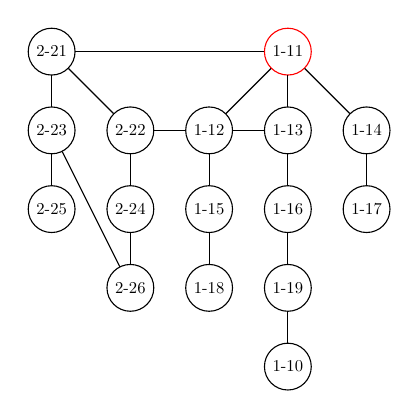
\begin{tikzpicture}
			\tikzstyle{AS}=[circle,draw=black,scale=0.6]
			\begin{scope}
			\node[AS,draw=red] (1-11) at (0,0)   {1-11};
			\node[AS] (1-12) at (-1,-1) {1-12};
			\node[AS] (1-13) at (0,-1)  {1-13};
			\node[AS] (1-14) at (1,-1)  {1-14};
			\node[AS] (1-15) at (-1,-2) {1-15};
			\node[AS] (1-16) at (0,-2)  {1-16};
			\node[AS] (1-17) at (1,-2)  {1-17};
			\node[AS] (1-18) at (-1,-3) {1-18};
			\node[AS] (1-19) at (0,-3)  {1-19};
			\node[AS] (1-10) at (0,-4)  {1-10};
			
			\node[AS] (2-21) at (-3,0)   {2-21};
			\node[AS] (2-22) at (-2,-1)  {2-22};
			\node[AS] (2-23) at (-3,-1)  {2-23};
			\node[AS] (2-24) at (-2,-2)  {2-24};
			\node[AS] (2-25) at (-3,-2)  {2-25};
			\node[AS] (2-26) at (-2,-3)  {2-26};
			\end{scope}
			
			\path[-]    
			(1-11) edge (1-12) 
			(1-11) edge (1-13)
			(1-11) edge (1-14)
			(1-12) edge (1-13)
			(1-12) edge (1-15)
			(1-13) edge (1-16)
			(1-14) edge (1-17)
			(1-15) edge (1-18)
			(1-16) edge (1-19)
			(1-19) edge (1-10)
			
			(1-11) edge (2-21)
			(1-12) edge (2-22)
			(2-21) edge (2-22)
			(2-21) edge (2-23)
			(2-22) edge (2-24)
			(2-23) edge (2-25)
			(2-23) edge (2-26)
			(2-24) edge (2-26)
			;
		\end{tikzpicture}
		\caption{Logarithmic, b=10}
		\label{fig:main:concept:scaling:log2}
	\end{subfigure} 
	\hfill
	\begin{subfigure}{.3\linewidth}
		\centering
		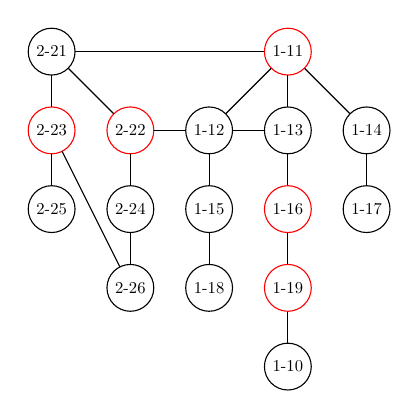
\begin{tikzpicture}
			\tikzstyle{AS}=[circle,draw=black,scale=0.6]
			\begin{scope}
			\node[AS,draw=red] (1-11) at (0,0)   {1-11};
			\node[AS] (1-12) at (-1,-1) {1-12};
			\node[AS] (1-13) at (0,-1)  {1-13};
			\node[AS] (1-14) at (1,-1)  {1-14};
			\node[AS] (1-15) at (-1,-2) {1-15};
			\node[AS,draw=red] (1-16) at (0,-2)  {1-16};
			\node[AS] (1-17) at (1,-2)  {1-17};
			\node[AS] (1-18) at (-1,-3) {1-18};
			\node[AS,draw=red] (1-19) at (0,-3)  {1-19};
			\node[AS] (1-10) at (0,-4)  {1-10};
			
			\node[AS] (2-21) at (-3,0)   {2-21};
			\node[AS,draw=red] (2-22) at (-2,-1)  {2-22};
			\node[AS,draw=red] (2-23) at (-3,-1)  {2-23};
			\node[AS] (2-24) at (-2,-2)  {2-24};
			\node[AS] (2-25) at (-3,-2)  {2-25};
			\node[AS] (2-26) at (-2,-3)  {2-26};
			\end{scope}

			\path[-]    
			(1-11) edge (1-12) 
			(1-11) edge (1-13)
			(1-11) edge (1-14)
			(1-12) edge (1-13)
			(1-12) edge (1-15)
			(1-13) edge (1-16)
			(1-14) edge (1-17)
			(1-15) edge (1-18)
			(1-16) edge (1-19)
			(1-19) edge (1-10)
			
			(1-11) edge (2-21)
			(1-12) edge (2-22)
			(2-21) edge (2-22)
			(2-21) edge (2-23)
			(2-22) edge (2-24)
			(2-23) edge (2-25)
			(2-23) edge (2-26)
			(2-24) edge (2-26)
			;
		\end{tikzpicture}
		\caption{Linear, x=0.33}
		\label{fig:fig:main:concept:scaling:lin2}
	\end{subfigure}  
	\caption{Scaling strategies}
	\label{fig:main:concept:scaling}
\end{figure}

\subsubsection{Select SpeedCams} \label{sec:main:selectionPhase:selecting}

The selection of SpeedCam from the candidates itself is a forward process. Iterate over all nodes, generate a random number\footnote{It is sufficient for this work to use a weak pseudo random generator} from 0 to 1 (exclusive) $p$ and if $P_{sc}(n) \geq p$, than add the node $n$ to the selected set. The iteration if over, when there enough speed cams are selected.

The order of the candidates matters, because $k$ limits the size of the target set. This problem is shown in \autoref{fig:main:candidateSelectionOrder}. In \autoref{fig:main:selectionSorted} they are sorted by their probability. The loop starts at candidate with the highest probability. The chance, that $p$ is high enough that $n$ is selected, is higher for later $n$. Concluding from this, the chance for $n=3$ to become a SpeedCam is lower in case \autoref{fig:main:selectionSorted} than in the case \autoref{fig:main:selectionUnsorted}. Because of time constrains for this work, this change is not evaluated.
\begin{figure}[h]
    \begin{subfigure}{.45\linewidth}
        \centering
        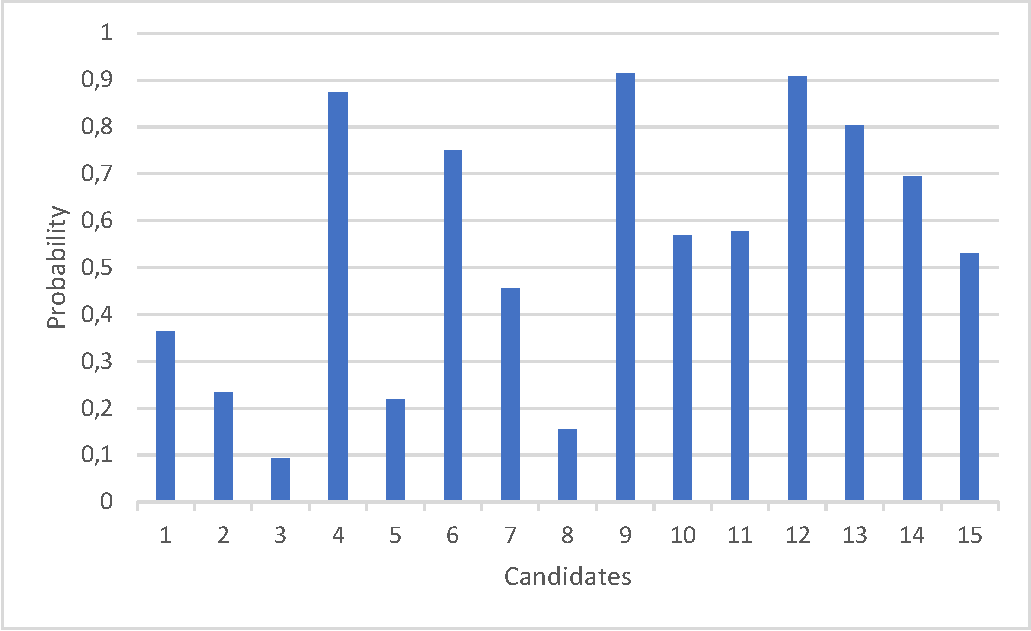
\includegraphics[trim={3mm 3mm 3mm 3mm},clip,width=0.8\textwidth]{selectUnsortedPlot.pdf}
        \caption{Unsorted}
        \label{fig:main:selectionUnsorted}
    \end{subfigure}%
    \begin{subfigure}{0.45\linewidth}
        \centering
        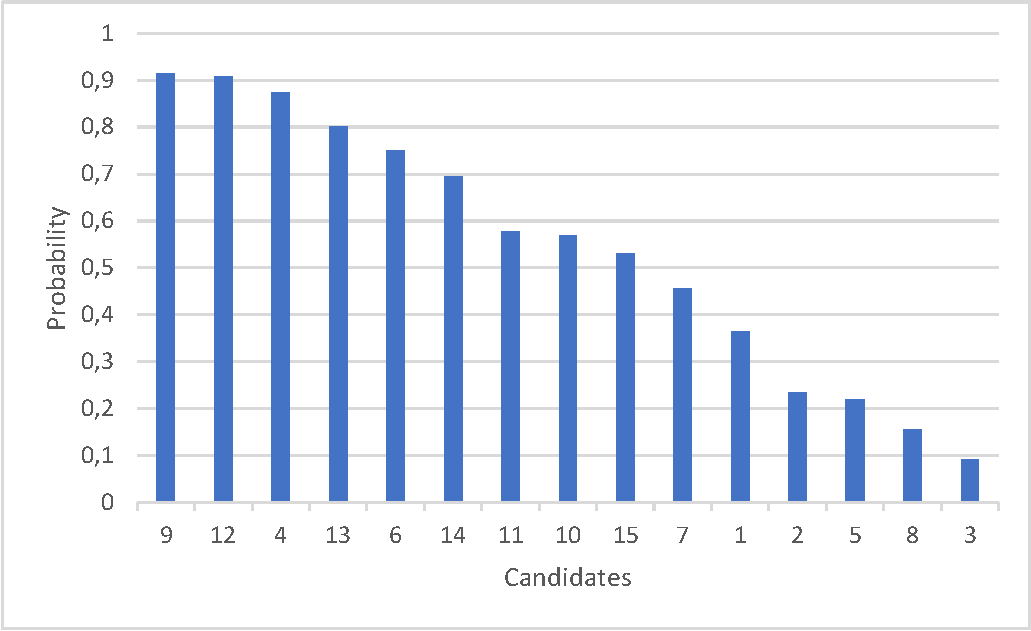
\includegraphics[trim={3mm 3mm 3mm 3mm},clip,width=0.8\textwidth]{selectSortedPlot.pdf}
        \caption{Sorted by probability}
        \label{fig:main:selectionSorted}
    \end{subfigure}
    \caption{Example of detection scheme}
    \label{fig:main:candidateSelectionOrder}
\end{figure}

The selection phase ends with a set of $k$ nodes, which are functioning for the next phases as \textbf{SpeedCams}.

\subsection{Monitoring} \label{sec:main:monitoringphase}
The monitoring uses the set of nodes from the Selection phase, which are now called SpeedCams. They have the task to log the transferred traffic over a timespan from $t_1$ to $t_2$. At the end of that timespan, they need to report the results to the inspector. There are different resolutions for the logged traffic, which are visualized in conceptually in \autoref{fig:main:concept:monitoring}. A red outline represents a probe and a blue color represents the possibility to measure traffic.

\begin{figure}[h]
	\centering
	\begin{subfigure}{.3\linewidth}
		\centering
		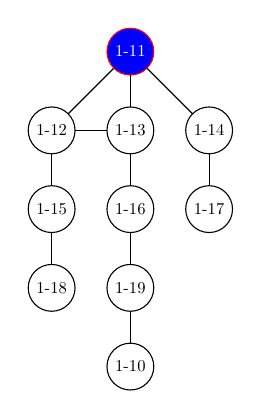
\begin{tikzpicture}
		\tikzstyle{AS}=[circle,draw=black,scale=0.6]
		\node[AS,draw=red,fill=blue,text=white] (1-11) at (0,0) {1-11};
		\node[AS] (1-12) at (-1,-1) {1-12};
		\node[AS] (1-13) at (0,-1)  {1-13};
		\node[AS] (1-14) at (1,-1)  {1-14};
		\node[AS] (1-15) at (-1,-2) {1-15};
		\node[AS] (1-16) at (0,-2)  {1-16};
		\node[AS] (1-17) at (1,-2)  {1-17};
		\node[AS] (1-18) at (-1,-3) {1-18};
		\node[AS] (1-19) at (0,-3)  {1-19};
		\node[AS] (1-10) at (0,-4)  {1-10};

		\path[-]    
		(1-11) edge (1-12) 
		(1-11) edge (1-13)
		(1-11) edge (1-14)
		(1-12) edge (1-13)
		(1-12) edge (1-15)
		(1-13) edge (1-16)
		(1-14) edge (1-17)
		(1-15) edge (1-18)
		(1-16) edge (1-19)
		(1-19) edge (1-10)
		;
		\end{tikzpicture}
		\caption{Node}
		\label{fig:main:concept:monitoring:node}
	\end{subfigure}
	\hfill
	\begin{subfigure}{.3\linewidth}
		\centering
		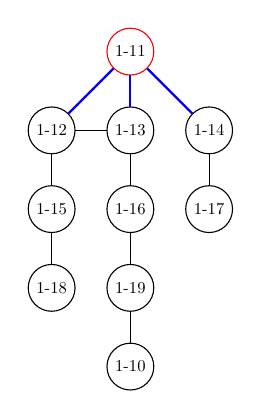
\begin{tikzpicture}
		\tikzstyle{AS}=[circle,draw=black,scale=0.6]
		\begin{scope}
		\node[AS,draw=red] (1-11) at (0,0)   {1-11};
		\node[AS] (1-12) at (-1,-1) {1-12};
		\node[AS] (1-13) at (0,-1)  {1-13};
		\node[AS] (1-14) at (1,-1)  {1-14};
		\node[AS] (1-15) at (-1,-2) {1-15};
		\node[AS] (1-16) at (0,-2)  {1-16};
		\node[AS] (1-17) at (1,-2)  {1-17};
		\node[AS] (1-18) at (-1,-3) {1-18};
		\node[AS] (1-19) at (0,-3)  {1-19};
		\node[AS] (1-10) at (0,-4)  {1-10};
		\end{scope}
		
		\path[-]    
		(1-11) edge[draw=blue, style=thick] (1-12) 
		(1-11) edge[draw=blue, style=thick] (1-13)
		(1-11) edge[draw=blue, style=thick] (1-14)
		(1-12) edge (1-13)
		(1-12) edge (1-15)
		(1-13) edge (1-16)
		(1-14) edge (1-17)
		(1-15) edge (1-18)
		(1-16) edge (1-19)
		(1-19) edge (1-10)
		;
		\end{tikzpicture}
		\caption{Link}
		\label{fig:main:concept:monitoring:link}
	\end{subfigure}
	\hfill
	\begin{subfigure}{.3\linewidth}
		\centering
		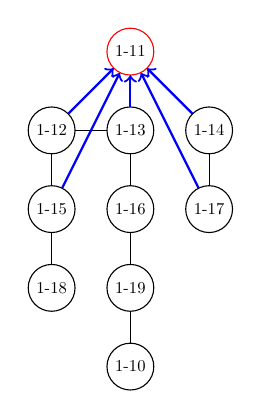
\begin{tikzpicture}
		\tikzstyle{AS}=[circle,draw=black,scale=0.6]
		\begin{scope}
		\node[AS,draw=red] (1-11) at (0,0)   {1-11};
		\node[AS] (1-12) at (-1,-1) {1-12};
		\node[AS] (1-13) at (0,-1)  {1-13};
		\node[AS] (1-14) at (1,-1)  {1-14};
		\node[AS] (1-15) at (-1,-2) {1-15};
		\node[AS] (1-16) at (0,-2)  {1-16};
		\node[AS] (1-17) at (1,-2)  {1-17};
		\node[AS] (1-18) at (-1,-3) {1-18};
		\node[AS] (1-19) at (0,-3)  {1-19};
		\node[AS] (1-10) at (0,-4)  {1-10};
		\end{scope}
		
		\path[-]    
		(1-11) edge (1-12) 
		(1-11) edge (1-13)
		(1-11) edge (1-14)
		(1-12) edge (1-13)
		(1-12) edge (1-15)
		(1-13) edge (1-16)
		(1-14) edge (1-17)
		(1-15) edge (1-18)
		(1-16) edge (1-19)
		(1-19) edge (1-10)
		;
		\path[<-]
		(1-11) edge[draw=blue, style=thick] (1-12) 
		(1-11) edge[draw=blue, style=thick] (1-13)
		(1-11) edge[draw=blue, style=thick] (1-14)
		(1-11) edge[draw=blue, style=thick] (1-15)
		(1-11) edge[draw=blue, style=thick] (1-17)
		;
		
		\end{tikzpicture}
		\caption{Flow}
		\label{fig:main:concept:monitoring:flow}
	\end{subfigure}
	
	\caption{Monitoring resolution}
	\label{fig:main:concept:monitoring}
\end{figure}
The lowest resolution is to summarize the in- and outgoing traffic of the node  (\autoref{fig:main:concept:monitoring:node}). This resolution is simple to implement and produces the smallest amount of footprint, because it needs only one counter per node. But it leaks in details and limits the possibility of the SpeedCam.

The next resolution is higher and logs the traffic per link separately  (\autoref{fig:main:concept:monitoring:link}). The advantage over the previous resolution is that it is not only possible to log the activity of the node itself by aggregating all link traffics. It gives the possibility to also log a fraction of traffic from the neighbours node. The disadvantage is that each link has to be monitored and there is a counter needed for each link. This results in a higher footprint.

A higher resolution of the monitoring is achievable by also looking at a packets metadata. The previously resolutions only aggregates the packet sizes, while this packets inspection enables the SpeedCam to construct flows  (\autoref{fig:main:concept:monitoring:flow}). With that information it is possible to not only reconstruct the neighbours traffic, but also the sender and receiver traffic. This approach has a higher footprint, because it needs to count the traffic for each node pair.

The choice of resolution is based on the amount of available computation power and the possibilities of the network type itself. The current Internet uses the OSI layer \todo{Quelle} and when the inspector is using the application layer, it cannot access the necessary information for higher resolutions. The chosen resolution for this work is explained in \autoref{sec:main:scionimpl}.

The results of the SpeedCams are sent to the inspector and will be processed by him in the next phase, the conclusion.

\subsection{Conclusion} \label{sec:main:conclusionphase}
The conclusion uses the information from the monitoring phase about the logged traffic from the SpeedCams. The goal of that phase is to aggregate the traffic and reconstruct the flow inside the network to identify a misuse of network resources. It also back feeds the results to the graph and ends the episode.

The inspector receives the measured traffics from the SpeedCams and aggregates them in such a way, that the inspector can add them to the corresponding node. After this assignment, the inspector decides, which node violated the rules. To do so, he needs to classify the users, which is described in the following:

The classification of the a node depends on two factors: The first one is if the inspectee violated the rule and overused its limits. The second one is if there was a \textit{congestion} inside the network, so that one node was constantly at its bandwidth limit and unable to fulfil its task. The resulting cases are shown in \autoref{tab:classifyUser}.

\begin{table}[h]
    \centering
    \begin{tabular}{ r|c|c| }
        \multicolumn{1}{r}{}
        &  \multicolumn{1}{c}{no congestion}
        & \multicolumn{1}{c}{congestion} \\
        \cline{2-3}
        stays in limit & I & II \\
        \cline{2-3}
        overuses limit & III & IV \\
        \cline{2-3}
    \end{tabular}
    \caption{Classification of a node}
    \label{tab:classifyUser}    
\end{table}

\subsubsection{Case I - Fair} \label{sub:main:detection:case1}
This node uses fewer bandwidth than he has subscribed to and doesn't violate the rule. There is also no congestion inside the network. In this case, there is no need to punish the user. They could use even more bandwidth, because the network is currently underutilized and possible bandwidth is wasted.

\subsubsection{Case II - Global greedy}
In this case there is a congestion inside the network. The currently used bandwidth is higher than the available. But there is not any node which violated the rule. This results in a global greedy behaviour of all nodes, because their cumulative task needed more resources than were available.  Because of the missing culprit the punishment is not as easy as in case 4.

It is possible to resolve this case for future episode by identifying the nodes with the highest bandwidth and to plea them not using so much resources. They can identified by \textit{clustering-algorithm}, such as \textit{Jenks Natural Breaks}\todo{Quelle dafür}. This would be a type of \textit{load-balancing}, but it is in a network difficult to realize. The nodes owner maybe paid for the subscribed bandwidth and will ignore to such a plea. All in all it is only possible to identify the global greedy nodes, but it is outside this work to go into detail.

\todo{Add figure to display the issue}

\subsubsection{Case III - Overusing with no congestion}
This case occurs when there is no congestion, but a  node uses more bandwidth than it has subscribed for. For example, a node has only a subscription for 1 GBit/s, but uses 1.2 GBit/s. The difference to case IV is, that beside overusing, it does not result in a congestion.

On the one hand this behaviour can quickly lead to a congestion when every node behaves like this. On the other hand this behaviour utilizes the bandwidth in a better way, because otherwise the unused capacity would be wasted.

The node is classified as greedy, but do not need to be punished immediately. A better way would be to tolerate a certain percentage of overuse and punish the user if he uses more than tolerated. The tolerance range would be 10\% without any problems. If the node uses more than 110\% of its bandwidth the node should be handled as in case IV user and receive a delayed punishment.

\todo{Add line graph to visualize this part}

\subsubsection{Case IV - Overuse resulted in a congestion}
The inspectee violated the limits and caused maybe with that behaviour a congestion. This node should be punished to prevent this in future episodes.

\subsection{Repeat} \label{sec:main:repeatphase}

\todo{Timeline example - 3 stück nebeneinander, im hintergrund ein verlauf des traffics}
The previously described phases need to be repeated in a certain interval. As with the other phases, there are several different strategies possible.

A \textit{fixed interval} with an endless repeat mode is the first one. The inspector starts the inspection every $t$ time unit and gets a constant stream of information about the network traffics. The precision of the inspection depends on the size of the interval, the smaller the interval is, the higher is the precision. But also increases/decreases the resource impact. This strategy gives also the possibility for the inspectees to recognize this pattern and adapt.

A \textit{randomly chosen} time schedule prevents this problem. The inspector starts an inspection non-deterministic a few times over a given timespan, like a day or week. This decreases the precision of the measurement, because the interval changes randomly. The inspector looses the possibility to improve his selection quality by using the time profiles. This strategy can also waste the inspector resources, when the inspection is randomly chosen at a point of time with nothing happening of interest.

Another strategy is to utilize the knowledge of past episodes and the course of the traffic over a day. The inspector can check, if there are timestamps when the the traffic is usually high, for example in the evening for consumer \todo{Quelle für diesen Fakt finden}. This strategy is \textit{experiences based} and has the same advantages and issues as the \textbf{activity} criteria from \autoref{sec:main:selectionPhase:criteria}. A longer history enables more precise decision, but a too long history can hold outdated information. Also is a purely experienced based strategy vulnerable to get stuck in a local optima. This convergence can be avoided by using a chance to pick a non optimal timestamp to learn something new.

\subsection{Summary}
This section described the SpeedCam approach for general network and the different strategies. It is designed to work on any network, but quite so it lacks of necessary answers for questions like "Which components enables the inspector to measure traffic?" or "What protocols are necessary to exchange the monitored information?". The following section will show the example implementation in SCION and the section after especially for SCIONLab.

\section{Implementation in SCION} \label{sec:main:scionimpl}

This section will outline the implementation of the general concept as discussed in \autoref{sec:main:generalconcept}. SCION is under heavy development and hasn't reached a long-term-support (LTS) version yet. So it is necessary to mention, that the implementation was done with the version  24d2e97909599bf35dcbf6308aa2302610cf9689 from 2018-02-07T17:03:35Z. 

\subsection{Differences}

There are for this work interesting differences from the general networks to SCIONs structure. They will be shown in this part and used later for changes inside the phases. The nodes or inspectees will be now called ASes, because they are named so in SCION.

The first difference is, that there are core ASes inside one ISD. They are forming the core of an ISD and provides information about its structure. An AS which wants to find a path for his data sends a path-request to a core AS. The request responds contains up-down paths \todo{Bezeichnungen in SCION finden} from the source to the target AS. It is currently possible to log the path-server's requests. This information about active paths inside an ISD is useful for the exploration phase (\autoref{sec:main:explorationphase}), because it enables the inspector reconstruct the graph by adding all paths. There is no need to implement a graph exploring algorithm.

Based on that difference, the Core is a good place to insert the inspector. It needs to has access to the ISD and its structure and this is one of the tasks of the core. It would also be the place to enforce the policy, that the member of that ISD can be monitored and eventually be punished. 

Another useful difference is that an AS creates a new border router instance for each new link. Each instance collects the traffic metrics with the library Prometheus and provides them with a simple HTTP based protocol. The URL for the call can be bind to an open and externally accessible network interface. This fact simplifies the necessary implementation for the monitoring phase (\autoref{sec:main:monitoringphase}). It is also enables the resolution of link-based traffic, because each border router is responsible for one link. The work of Foster\cite{Forster.September2017} would count the bandwidth efficiently with a very small footprint, but until the used version his changes were not merged. 

The structure of SCION with ISD gives the possibility to split the responsibility for the inspection into multiple region, for example one inspector for each ISD. This will improve the scalability of the Inspector, but implementing it as a decentralized component would go beyond the scope of this work.

The next section will give an overview about the implementation using SCION as its network without going into detail about code fragments. Any approaches or algorithms in the implementation were explained in previous section and the posting of Go code fragments do not yield any additional advantage, when they can be found on the repository itself.

\section{Implementation in SCIONLab} \label{sec:main:scionlabimpl}

The implementation\footnote{\url{https://github.com/Meldanor/SCIONLab_SpeedCam}, 05.04.2018} was mostly written in Go\footnote{\url{https://golang.org}, 05.04.2018} 1.9. SCION itself and most of its component are written in Go and because of that is made sense to also write the implementation in Go. The amount of components very specific to Go is limited and was written in an object-oriented way to be portable to other programming languages. It also uses as few SCION dependencies as possible to be lightweight and flexible to use. The implementation is sufficient enough for this work and should not be used in its current state in a production environment, but it can be used as a base for a production ready application. The documentation for this program can be found in the README.md of the project as also in \autoref{app:usage}

An overview about the communication between the implemented components and their corresponding phases is given as an UML communication diagram in \autoref{fig:main:impl:phasescommunication}. Each phase and its specific communication is numbered, starting with 0 for the exploration phase. This phase is completely executed in the background. The other phases, methods starting with 1, 2 and 3 are run in sequence. In the following of this part, each method will be explained in detail and any difference from the concept, if existing, is mentioned.

\begin{figure}
	\centering
	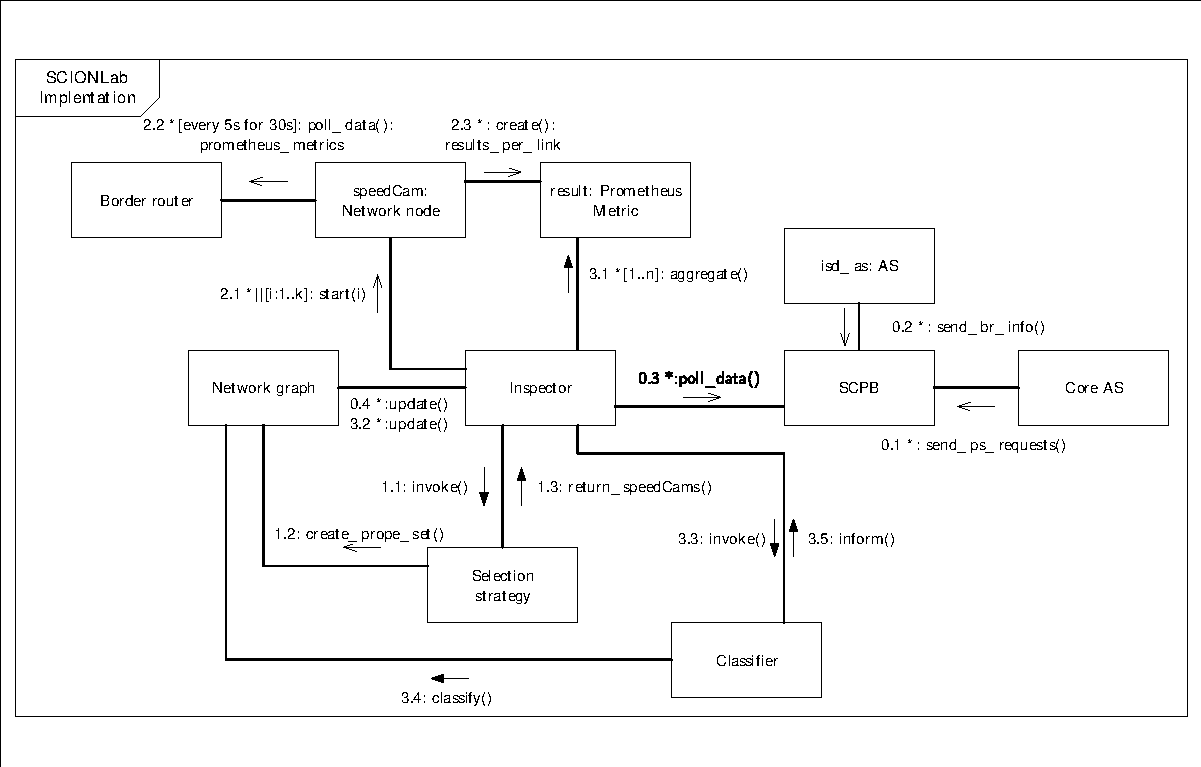
\includegraphics[trim=0.1in 0.2in 0 0.2in, clip, width=0.95\textwidth]{umldiagram_scionLabImpl_communication.pdf}
	\caption{SCIONLab implementation - communication diagram}
	\label{fig:main:impl:phasescommunication}
\end{figure}

The Prometheus metrics are published via a REST resource. Therefore, the inspector needs to know the URL of the border router. This information is stored on the AS itself and not externally available for security reasons. The solution for this problem was to create two components. The first one is a script written by Kwon, Jonghoon to parse the border router configuration file and extracts the Prometheus URL. The script itself is deployed to each AS. This information is send to the second component, the \textbf{S}peed\textbf{C}am\textbf{P}rometheus\textbf{B}ridge (SCPB) server program\footnote{\url{https://github.com/Meldanor/SCPB}, 05.04.2018}. This in Java written application is a RESTful service to receive and serve information about Prometheus clients. It was originally written to add monitoring targets to the local running Prometheus server. In the progress of this thesis it was extended to not only handle Prometheus client information, but also temporary store Path server requests and make them available to the inspector. This behaviour is shown in \autoref{fig:main:impl:phasescommunication}.
(0.1) The script is sending the border router information, (0.2) another script\footnote{\url{https://github.com/Meldanor/SCIONLab_SpeedCam/blob/master/ps_request_parser/ps_request_parser.go}, 05.04.2018} parses the path server requests on a core AS and both send this data to the REST resources of SCPB. (0.3) The inspector polls this data in an interval to (0.4) update his network graph. The exploration phase is done asynchronously and repeats every minute.

The selection phase was implemented as described in \autoref{sec:main:selectionPhase}. The inspectors starts an episode and (1.) invokes the given selection strategy. Depending on the strategy it (2.) creates a set of probes by selecting the best candidates. The candidate score is missing the \textit{capacity} information about a link. There is an attribute assigned by SCION, but in SCIONLab it was set inconsistently and therefore was unreliable. Currently, SCION itself does not make use of this attribute. In conclusion the capacity is for each node 1 and the \textit{activity} is simply the average bandwidth of the link.
The order of the candidates, as described in \autoref{sec:main:selectionPhase:selecting} does have an impact on the chance to be selected. This implementation uses the random order instead of the sorted, because there is no standard implementation of Go maps, which are sorted by there keys \cite{goMapsInAction.2013}.

With the set of ASes to probe, (2.1) the inspector will construct SpeedCams and pass them the information for their border router to fetch data from. This starts the monitoring phase (\autoref{sec:main:monitoringphase}). (2.2) The SpeedCams run simultaneously in separate Goroutines for 30s each and requests data every 5s seconds. The URL of the request is \lstinline|http://[BORDER_ROUTER_IP]:[PROMETHEUS_PORT]/metrics|. The respond of the resource is a text formatted file forming a key-pair list. For the border router, the keys \textit{border\_input\_bytes\_total} for the ingress traffic and \textit{border\_output\_bytes\_total} for the egress traffic of this border router. Each value is a cumulative value continuously increasing over time and stored as a 64 bit floating point value. The bandwidth, bytes per second, is differentiated by using calculating the difference quotient (2.3). The arithmetic error can be reduced by narrowing down the scrap interval, but this would increase the necessary computation power and, due to more network called, also the used bandwidth.

For the conclusion phase (\autoref{sec:main:conclusionphase}) the inspector needs to aggregate the data (3.1). The recorded bandwidth per link is averaged and added to the activity of both nodes of the link (3.2). The classifier is invoked (3.3) by the inspector with the updated graph. It starts to classify the nodes of the network based on the new data (3.4) and inform the inspector about it. For the evaluation of this work, the results of this episode are written to a JSON file. It contains the graph in its current state, the configuration of the program and the list monitored results per link. This ends the conclusion phase and the episode. The next episode is started by the inspector after  $n$ seconds, depending on the selected strategy as described in \autoref{sec:main:repeat}.

\section{Summary}
This chapter introduced the SpeedCam approach based on the inspection game. At first a general concept for an efficient, decentralized monitoring was given, which can be applied to any kind of network. It was split into five phases to construct the network graph, to select probes, to monitor the traffic on the probes and to classify the nodes. Each of the phases can be executed by different strategies, which were also discussed. The general concept was adapted to SCION and implemented in SCIONLab for the evaluation of the discussed strategies. This will be shown in the next chapter.
\subfilebib % Makes bibliography available when compiling as subfile
\end{document}